% 图 1.3 磁场 B 中的磁矩 mu（夹角 theta）
\documentclass[tikz,border=5pt]{standalone}
\usetikzlibrary{arrows.meta}
\usepackage{amsmath}
\usepackage{bm}
\usepackage{fontspec}
\setmainfont{Times New Roman}
\begin{document}
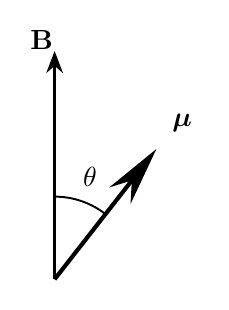
\begin{tikzpicture}[line width=1.0pt,>=Stealth]
% 磁场 B
\draw[->,line width=1.1pt] (0,0) -- (0,2.9)
  node[pos=1,above left=-1pt,inner sep=1pt] {$\mathbf{B}$};
% 磁矩 mu（粗偶极针）
\draw[line width=1.5pt,-{Stealth[length=7.5mm,width=3.4mm]}]
  (0,0) -- (52:2.1);
\node at (1.62,1.98) {$\boldsymbol{\mu}$};
% 夹角 theta
\draw[line width=0.7pt] (90:1.05) arc[start angle=90,end angle=52,radius=1.05];
\node at (71:1.38) {$\theta$};
\end{tikzpicture}
\end{document}
